
%\subsubsection{ECal Trigger overview}




The signals from the from top and bottom parts of the ECal and muon system will be sent to the FADC boards, located in VXS crates. Two VXS crates are needed to accommodate all channels from the ECal and one for the muon system. 
As mentioned above the FADC digitizes the measured pulse height (with 12-bits) of each ECal and muon channel every 4~ns for further trigger and readout processing. The FADC sends the information about the pulse energy and time to the Crate Trigger processor (CTP). Thus, the first stage of the trigger logic are incorporated into the FPGA firmware on the FADC boards. 
%The final trigger decision, based on information from both halves of the ECal and the muon system are built using the CTP and finally the Sub-System Processor (SSP).

The trigger system for the ECal can be broken down into three sections, see Fig.~\ref{fig:hps_trigger_cal}:
 \begin{itemize}
 \item FADC (pulse finding): Samples and digitizes the signal pulses from each detector channel. It sends the measured pulse energy and arrival time to the CTP.
 \item CTP (cluster finding): Group channels from the FADC into clusters. The cluster energy, arrival time, and hit pattern are sent to Sub-System Processor (SSP).
 \item SSP (cluster pair finding): Find pairs of clusters from the CTP (from top and bottom halves of the detector) and applies topological selections. Generates the final trigger decision for events fulfilling the pair selection.
 \end{itemize}
\begin{figure}[t]
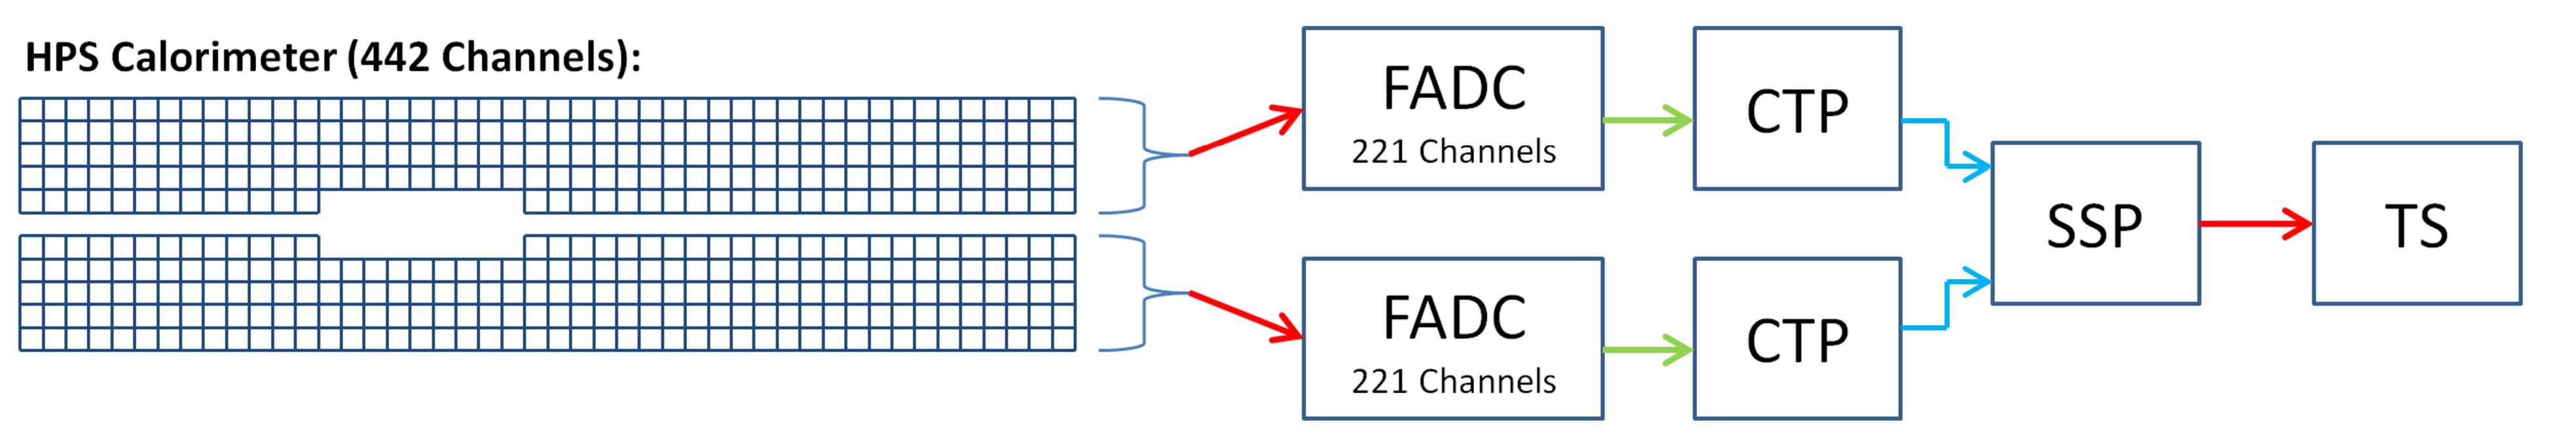
\includegraphics[scale=0.25]{daq_trigger/figures/hps_trigger_cal}
\caption{\small{Block diagram of the ECAL trigger system consisting of the FADC that digitizes the detector channels signals and sends them for cluster finding in the Crate Trigger Processor (CTP). The found clusters are sent to the Sub-System Processior (SSP). The final trigger decision, based on pairs in both halves of the ECal, is built in the SSP and sent to the Trigger Supervisor for further distribution to all the sub-systems.}}
\label{fig:hps_trigger_cal}
\end{figure}
The trigger search for a time coincidence between two clusters in opposite halves of ECal that occur within a programmable time window with 4~ns resolution. The maximum trigger decision time, or trigger latency, is set to match the latency needed for the SVT APV25 chip, 
$\sim3\mu$. The Trigger Supervisor receives information on a trigger accept from the SSP and generates all necessary signals. It controls the entire DAQ system readout through theTrigger Interface units installed in every crate that participates in the readout process. The system is free-running based on the 250~MHz master clock and has essentially no dead time. An artificial dead time, e.g. after a 'busy' from the front-end electronics, can be generated by the trigger supervisor. The maximum trigger accept rate is $>50$~kHz.




%\subsubsection{Crate Trigger Processor} 

The CTP receives the pulse energy (in MeV) and time stamp from each FADC channel in the crate.
The algorithm used for cluster finding makes use the parallel processing nature of FPGAs by simultaneously searching for 125 clusters up to 3x3 in size across the calorimeter crystal array, see 
Fig.~\ref{fig:hps_trigger_3x3}. 
\begin{figure}[h]
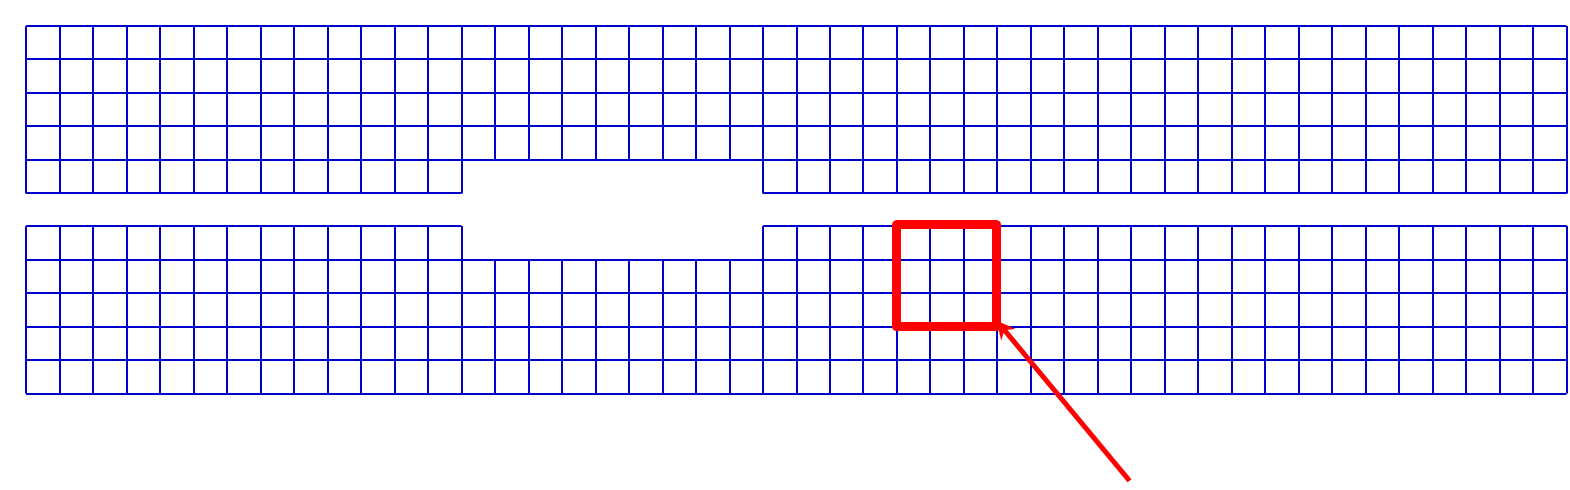
\includegraphics[scale=0.4]{daq_trigger/figures/hps_trigger_3x3}
\caption{\small{Cluster finding algorithm.}}
\label{fig:hps_trigger_3x3}
\end{figure}
The clustering algorithm implemented in the CTP for the ECal:
\begin{itemize}
\item adds energy from hits together for every 3x3 square of channels in ECal,
\item add hits together if they occur (using the leading edge of the pulse) within a programmable number of 4~ns clock cycles of each other,
\item checks if the 3x3 energy sum is larger than the programmable cluster energy threshold,
\item  reports the time, energy, position and 3x3 hit pattern of the cluster to the SSP.
\end{itemize}
The CTP evaluates all hits, satisfying the programmable time coincidence, in the crate every 4~ns. This is done by reporting hits when they occur and then reporting them again for the next N number of 4~ns clock period, where N can be 0 to 7. This is useful to deal with skew and jitter that develop from the detector, cabling, and electronics. The CTP will only report a cluster to the SSP if the energy is greater than all neighboring (up, down, left, right, and diagonals) 3x3 cluster energies for that clock cycle. This filtering 
is applied since there are several 3x3 windows that overlap and also many physics single clusters are larger than a 3x3 window. The reported cluster information to the SSP is: the 13-bit cluster energy (in MeV), the cluster position (crystal index: x,y), the cluster time (with 4~ns resolution) and the cluster 3x3 hit pattern (channels reporting a hit in the cluster).
%\begin{itemize}
%\item 13bit Cluster energy (MeV)
%\item Cluster position (crystal index: x,y)
%\item Cluster time (4ns resolution)
%\item Cluster hit pattern 3x3 (detector channels reporting a hit in the cluster)
%\end{itemize}
The cluster position is the coordinate of the crystal with the maximum energy in the 3x3 window. The 3x3 cluster hit pattern can be used by the SSP to filter out strange clusters and/or make a low resolution cluster centroid computation.





%\subsubsection{Sub-System Processor} 

%The cluster's time, energy, position and 3x3 pattern found in two VXS crates are reported to the Sub-System Processor. 
The SSP collects cluster information from the full calorimeter and creates two types of triggers: single and pair trigger. The single cluster trigger includes programmable minimum and maximum cluster energy selections. The pair trigger is more elaborate and includes more selections based on topological information optimized to reject background events while keeping the trigger efficiency for A$^{\prime}$ events high. The programmable selections on the pair cluster candidates include:
\begin{itemize}
\item Energy sum,  
$E_{min}\le E_{top}+E_{bottom}\le E_{max}$
\item Pair time coincidence, 
$|t_{top}-t_{bottom}|\le \Delta t_{max}$ 
\item Energy difference, 
$|E_{top}-E_{bottom}|\le \Delta E_{max}$ 
\item Energy slope,
$E_{cluster\_with\_min\_energy}+R_{cluster\_with\_min\_energy}\times F_{energy}\le Threshold_{slope}$
\item Co-planarity, 
$|
tan^{-1}(\frac{X_{top}}{Y_{top}})-
tan^{-1}(\frac{X_{bottom}}{Y_{bottom}}) |\le Coplanarity_{angle}$
\item Number of hits in 3x3 window, 
\#$hits_{3\times 3}\ge HitThreshold$
\end{itemize}
\noindent
where $ E_{max}$,  $\Delta t_{max}$, $ \Delta E_{max}$ , $Threshold_{slope}$, 
$F_{energy}$, $Coplanarity_{angle}$
and
$HitThreshold$ are programable parameters.
%Immediate verification of each trigger cut will be 
%Online event analysis will be provided to be compared against trigger event data for immediate verification (on each trigger cut: cluster energies, positions, timing, energy slope, coplanarity and hit threshold). 
With identical readout and trigger pulse processing very precise agreement can be expected between trigger and readout and can be used to verify the trigger selections online.





%\subsubsection{Diagnostic Tools}

The previous experience with a similar trigger system, but with simpler logic, showed that diagnostic tools are necessary to make sure that the system work as expected. Scalers will be implemented for every ECal channel to easily identify hot or dead channels; an example of such diagnostic tool is shown in Fig.~\ref{fig:dvcs_beam} 
from the previous version of the calorimeter. 
\begin{figure}[h]
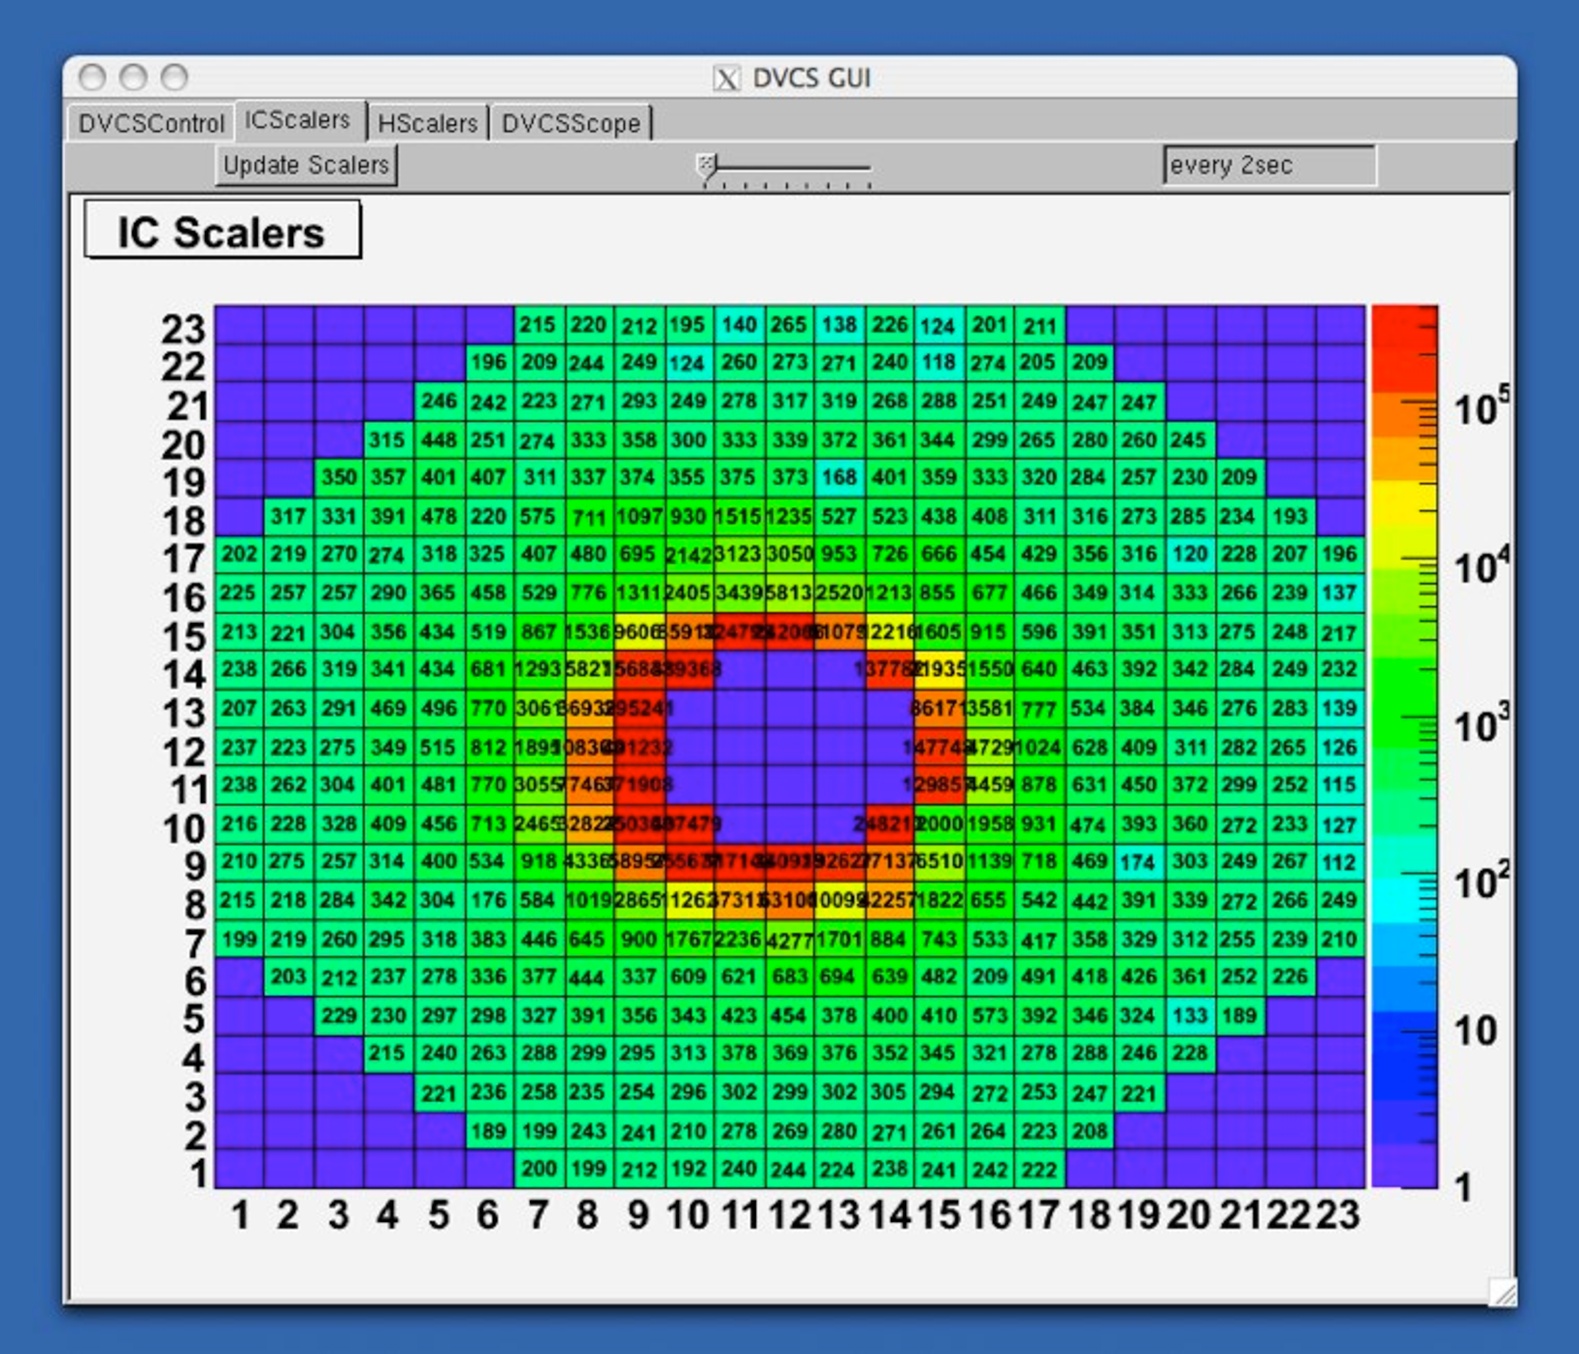
\includegraphics[scale=0.6]{daq_trigger/figures/dvcs_beam}
\caption{\small{Scalers (example from the previous version of the calorimeter).}}
\label{fig:dvcs_beam}
\end{figure}
A diagnostic scope will be used to analyze the trigger logic online. The goal to is to have a Two-Dimensional Analyzer 
to provide a debug interface which can identify bad channels, verify cluster finding algorithms and check timing. The customized logic analyzer runs in parallel, non-intrusive, to the calorimeter trigger and can setup a trigger 
on any ECal crystal arrangement and/or cluster counts and can move forward/backward in time by ~250 ns to understand timing details.
%\begin{itemize}
%\item Logic analyzer runs in parallel, non-intrusive, to the calorimeter trigger
%\item Can setup trigger on any ECal pixel arrangement and/or cluster count
%\item Can move forward/backward in time by ~250 ns to see timing details
%\item Will be customize for HPS geometry and hardware
%\end{itemize}
One example of the 2D logic analyzer can be seen in Fig.~\ref{fig:dvcs_2_cluster} from the previous version of the calorimeter.
\begin{figure}[]
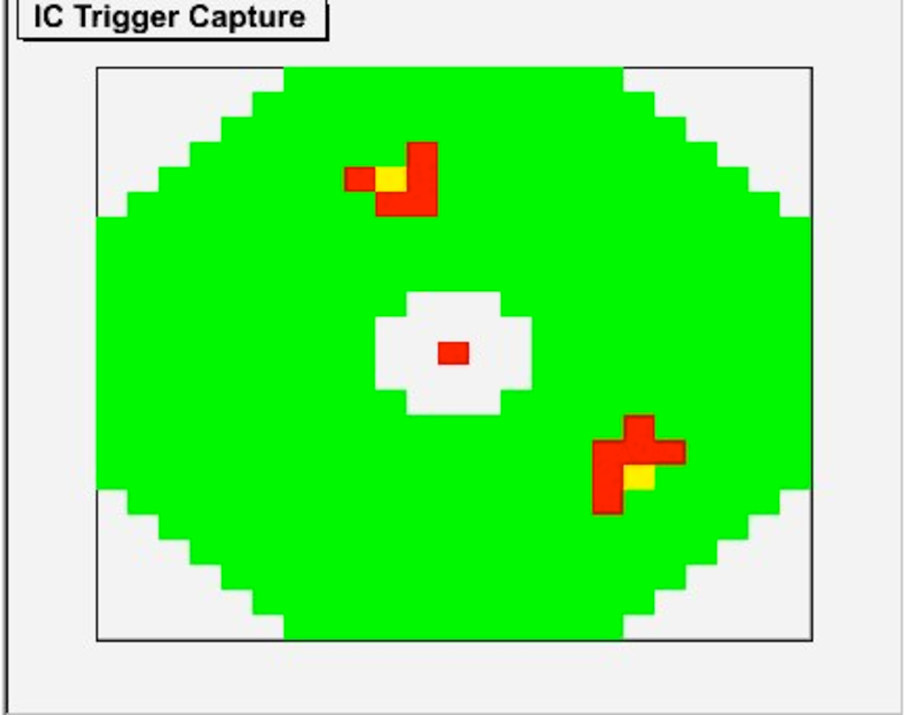
\includegraphics[scale=0.8]{daq_trigger/figures/dvcs_2_cluster}
\caption{\small{Example of the diagnostic scope of the ECal with two clusters found. This example is from the previous version of the calorimeter: green - no hits, red - tower with hit, yellow - cluster found.}}
\label{fig:dvcs_2_cluster}
\end{figure}
%Two clusters are displayed
%in the picture. The red color displays the hits in the calorimeter and  the center of clusters is displayed in yellow.
In addition to scalers, the distributions on individual pulse energy from each channel FADC channel will be monitored. 
To further debug the trigger chain, cluster positions and energy from SSP will be monitored and histograms with events that was accepted and rejected will be monitored for each trigger cut. 









%\subsubsection{Muon Trigger}

A muon detector composed of a four iron absorbers  and four double-layer scintillator planes, positioned after each absorber. Similar to the Ecal, the muon detector will consist of two halves, one above and one below the beam.
GEANT4 simulations have been used to study the trigger rates in the muon system due to background hits. It is expected that the true di-muon rate will be quite small compared to the ECal trigger rate and should not cause problem for the DAQ. 
A total of 144 readout channels are needed (9x16 channels multi-anode PMTs). Signals from each channel will be sent to a TDC and to a FADC. The FADC information will be used to construct the muon trigger. The TDC information together with information from FADC will be used in offline analysis to measure the hit position along the strip.

Selecting coincidence hits with MIP energy deposition in at least three layers of the scintillation hodoscope will identify muons. 
The muon trigger logic has to find one track in the top part of the detector in coincidence with another track in the bottom part of the detector. The track finding algorithm can be easily realized in the FPGA logic of the muon Crate Trigger processor.

